\section{Integration and Test Facility (ITF)}
\label{sec:fdsp-tc-itf}



The components of the \dword{dune} detectors will be manufactured in several different countries. 
Many of the parts can be reasonably shipped to the logistics warehouse and then underground where it can be installed. 
However, the  \dword{ce} and the \dwords{pd} are tightly coupled to the \dword{apa}s. 
The wires and filters on the d\dword{apa}s form part of the electronics circuit, and the photon supports and cabling are built into the \dword{apa}s. 
Integrating the \dword{ce} and \dword{pd}s into the \dword{apa}s is a huge task, and the risk of damaging the components is significant. Thus, we plan to integrate the components as early in the process as possible and then thoroughly test the complete assembly.
To avoid creating integration testing facilities at each factory, one central facility will be established in South Dakota near the \dword{surf} site  (within an hour's drive). 
The \dword{apa}s, \dword{ce}, and \dwords{pd} modules will arrive in this \dword{itf}, undergo initial tests, be integrated, and then undergo a set of warm tests. 

Because the \dword{ce} will be available approximately two years before installation begins, the \dword{itf} must be available on the same time scale. Other components are, in fact, available earlier. 
Table \ref{tab:specs:just:SP-TC} summarizes the specifications for the \dword{itf};  
the relevant specifications involve the quality of the cleanroom and the UV light filtering for the \dwords{pd}.



%\begin{dunetable}
%[ITF Specifications]
%{cc}
%{tab:tcps-itf-spec}
%{Summary of the high level specifications for the ITF. %The building requirements are covered separately in a separate section.}
%Parameter & Specification \\ \toprowrule
%Cleanroom & The ITF cleanroom shall meet ISO-8 standard per ISO-14644 \\ \colhline
%Filtered Lights & <520 nm for long exposure and <400 %for exposures less than 2 weeks \\ 
%\end{dunetable}



%%%%%%%%%%%%%%%%%%%%%%%%%%%%
\subsection{APA-CE-PD Integration}
\label{sec:fdsp-tc-itf-integ}

\begin{dunefigure}[ITF cleanroom layout]{fig:fdsp-tc-itf-clean}
{Conceptual layout of the cleanroom for APA-CE-PD integration and testing.}
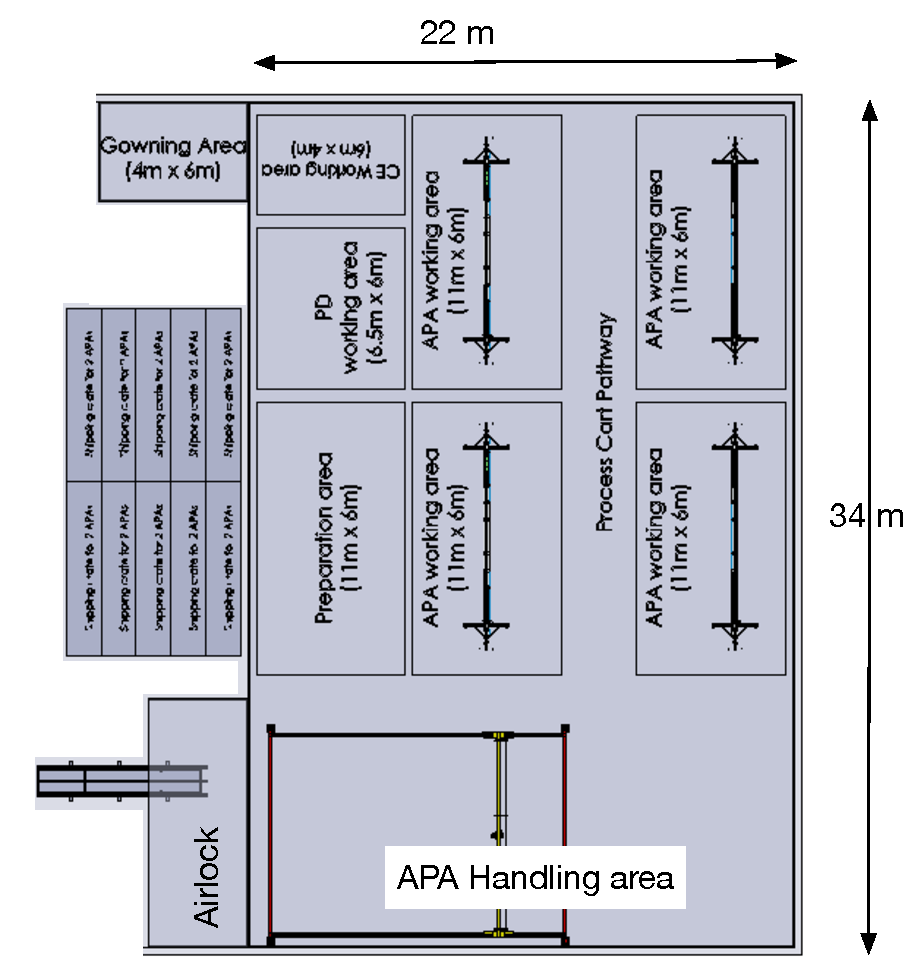
\includegraphics[width=0.8\textwidth]{itf-cleanroom-v2}
\end{dunefigure}

Most the work in the \dword{itf} must be done in a cleanroom environment to protect the components from dust and unfiltered light. The cleanliness requirement for the detector components is ISO-8 which corresponds to filtered air with clean lab coats, clean shoes, and hair nets. 
To protect the photon detector's \dword{wls} coating, the lights must be filtered to remove frequencies below 520nm.\cite{LBNE-docdb-8348} Figure \ref{fig:fdsp-tc-itf-clean} shows one possible layout of the cleanroom.
Materials enter the \dword{itf} cleanroom through the materials airlock. This area must be sufficiently large to accommodate \dword{apa} transport boxes and allow workers to move around the box to remove the dirty shipping layer and prepare the equipment for transport into the cleanroom. 
Other materials will also be brought into the cleanroom through the airlock, but they will need much less space than the \dword{apa} crates. Figure \ref{fig:fdsp-tc-itf-clean} shows an \dword{apa} transport box being moved into the airlock on the lower right.
The \dword{ce} and \dword{pd} equipment will be moved to their own work areas. 
Here the components are unpacked and tested before integration into the \dword{apa}. 
The tests performed are described in more detail in the \dword{qc}/\dword{qa} section below. 

The \dword{apa}s enter the cleanroom through the airlock and initially go to the \dword{apa} handling area where an overhead workstation or gantry crane will be available. 
The \dword{apa} will then be removed from the transport box and mounted to a process cart that can rotate the \dword{apa} horizontally. The process cart will be pushed to one of the four \dword{apa} integration areas where they are prepared for the installation of the \dword{ce} and \dword{pd}. 
During the integration process, the \dword{apa} will be held horizontal and the \dwords{pd} will be inserted into the sides while the \dword{ce} boxes are mounted to the end of the \dword{apa}. 
After integrating the components, the system will be tested and then moved back to the handling area and boxed for shipping to the logistics center for storage.  

All detector  components will arrive at the \dword{itf} either from the logistics facility or directly from the factories. Sufficient space will be needed inside the \dword{itf}, but outside the cleanroom, to store the material needed for several weeks as well as a few of the integrated \dword{apa} boxes. Additionally a changing room is needed, so workers can change into clean clothes and shoes. The changing room should have a capacity sufficient for the 10-20 workers needed in the cleanroom. 

%%%%%%%%%%%%%%%%%%%%%%%%%%%%
\subsection{ITF QA/QC}
\label{sec:fdsp-tc-itf-qaqc}
Extensive testing of the detector components will be performed inside the \dword{itf} facility as the APA-PD-CE integration takes place. These tests are a vital part of the quality control process for \dword{dune}. Details of the tests for each of the components are described below.

\subsubsection{APA}
The \dword{apa} will be unpacked from the transport box, installed on the process cart, and the protective shields removed to allow a detailed visual inspection. Then it will be transported to the integration area, where it will be held horizontally. The main test to be performed at this stage, i.e., before integration with the \dwords{pd} and \dword{ce}, is tension measurement. Ideally, all wires would be measured to ensure that no changes occurred during shipping. The limiting factor for the tension measurement will be time. In the current plan, approximately 350 wires, representing 10$\%$ of the total, will be measured, which will take 3 shifts with 2 people. All the measured values will be stored in the wire \dword{qc} database. In the current plan, the tension measurement will be performed using a laser, the same method used at the production site. This method uses a laser focused on individual wires. By plucking the wire to induce a vibration, a photodiode under the wire records the frequency of vibration, which directly translates into the tension value. While this method is robust and has been extensively used by \dword{lartpc} experiments, it is very time consuming. An alternative method, using electrical signals, is currently under development and could replace the laser method, potentially allowing all \dword{apa} wires to be measured at the \dword{itf} in less time.

The current requirement for tension values are 6$\pm$1 N. Wires measuring outside this range will be removed from the \dword{apa}. Note that the exact tolerance is currently under study with \dword{protodune} data to ensure the required acceptable range; otherwise, a channel may have to be removed.

The last test performed to ensure the quality of an \dword{apa} is the wire continuity. This checks that all wires are still intact and properly connected to the readout boards. This test can easily be done once the \dword{ce} is installed (see next sub-section).    
\subsubsection{Cold Electronics}
The \dword{qa} for the \dword{ce} is described in the \dword{ce} chapter.

\subsubsection{Photon Detectors}

\dwords{pd} will arrive at the \dword{itf} in custom designed crates.  Each crate will contain the ten photon detector modules required for a single \dword{apa}.  
Each \dword{pd} comes individually packaged in a static-resistant sealed plastic bag, filled with clean dry nitrogen.

Before each \dword{pd} is integrated into an \dword{apa}, it is removed from its shipping bag and inspected visually. 
Modules passing this initial inspection are then loaded into the optical scanner for operational testing.

The \dword{pd} optical scanner tests the operation of the photosensor readout chain to ensure all electrical connections are operational and also measures light-collection performance at several positions along the length of the module.  
Duplicate identical optical scanners are used at the module assembly facility, where a scan is the last \dword{qc} test before the module is shipped to the \dword{itf}; the module is tested again immediately before installation, allowing a sensitive test for any changes in module performance due to shipping or storage.  
This technique was used successfully in \dword{pdsp}, and will be replicated for \dword{dune}.

The optical scanner consists of a light-tight box, approximately \num{2.5}m long, with a \num{0.75} $\times$ \num{0.75}m cross section. 
The box is fabricated of aluminum and acts as a Faraday cage to minimize electrical interference with measurements. 
In the \dword{dune} configuration, two \dword{pd} modules to be tested are inserted into the station through slots on the face of the box, guided by support rails of the type used in the \dword{apa}s, representing a final mechanical check of the dimensions of the module.  
Electrical connection to the module uses an electrical connector identical to the ones in the \dword{apa} frames, allowing a final check of that crucial interface.
Following insertion into the scanner, the insertion slots are closed and optically sealed, and the scan begins. 
\dword{dune} \dword{pd} readout electronics are used to bias and read out the module photosensors, while a UV LED is scanned along the length of the modules by an automated stepper-motor driven translation stage.  
Measurements of the detector responses are made at 16 positions along the length of the module (on two sides for double-sided \dword{pd} modules), checking the performance of each of the dichroic filters. 
The response is compared to that measured in the assembly facility. 
Figure \ref{fig:fdsp-tc-pds-scanner} shows the scanner used to test the \dword{pdsp} photon detectors.


\begin{dunefigure}[Photon detector scanner]{fig:fdsp-tc-pds-scanner}
{Picture of the scanner for operational tests of the \dword{pd} modules before the modules are inserted into the \dword{apa}s.} 

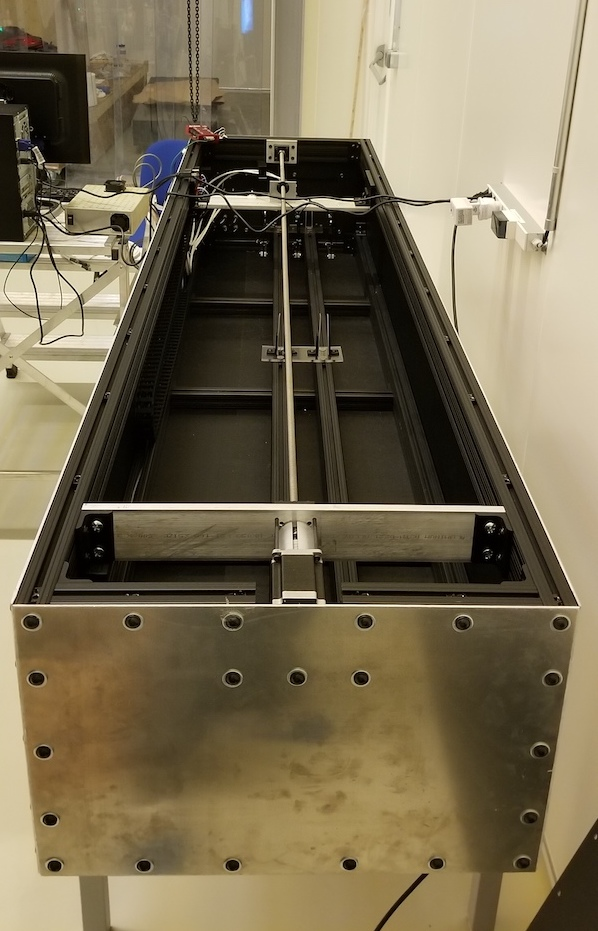
\includegraphics[height=.60\textheight, angle=0]{pds-scanner}
%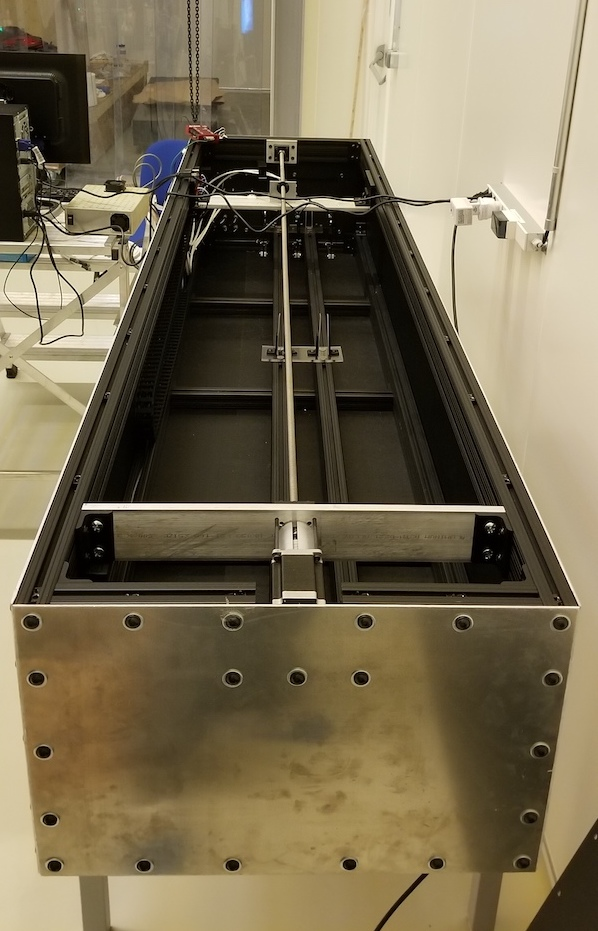
\includegraphics[width=1.0\textwidth, angle=-90]{pds-scanner}
\end{dunefigure}

Photon detector are inserted into the \dword{apa}s immediately follows optical scanning.  
Modules are inserted onto the \dword{pd} support rails; the connection to the cable harness, which is pre-installed in the \dword{apa} before wire wrapping, is automatic as the module is inserted.   
Immediately after the module is inserted, an electrical continuity check ensures continuity between the \dword{pd} module and the \dword{pd} cable end connector where it exits the end of the \dword{apa}.



%%%%%%%%%%%%%%%%%%%%%%%%%%%%
\subsection{Building Requirements and Infrastructure}
\label{sec:fdsp-tc-itf-req}
The \dword{itf} building requirements are summarized in DocDb 11500.\cite{bib:docdb11500} The building to be used as the \dword{itf} has not yet been designated. To help identify or design the \dword{itf} building, a set of requirements were drafted. The requirements document defines the spaces needed for integration work but does not specify the final layout of the cleanroom. This will allow cleanroom spaces to be configured as part of building footprints as candidate buildings are identified. Because the building has not been designated, the cleanroom layout shown in Figure \ref{fig:fdsp-tc-itf-clean} should be taken as a concept; the final layout may change depending on the footprint of the building chosen as the \dword{itf}. The building requirements document\cite{docdb-11500}  defines the minimum spaces needed for all operations inside the \dword{itf} cleanroom. It also defines the space needed for the coldbox and the related cryogenic system, and it provides guidance for the space needed for material storage outside the cleanroom. It also establishes requirements for power and other general needs. Some requirements depend on the location of the building and the facilities available in the area. For example, office space for 20 scientists working in the \dword{itf} will be needed in the area but would not necessarily need to be in the \dword{itf} building itself if other local options are available. Some local machining facilities also fall into this category. 

%%%%%%%%%%%%%%%%%%%%%%%%%%%%
\subsection{Safety}
\label{sec:fdsp-tc-itf-safety}

Information on \dword{itf} safety is identical to what is listed in Section 1.1.4 (Logistics Safety) because the \dword{itf} is also operated by SDSD as a Fermilab facility.    If the \dword{itf} and logistics facility are near each other, one safety officer can be shared by the two sites.    

%%%%%%%%%%%%%%%%%%%%%%%%%%%%
\subsection{Cost, Schedule and Risk Analysis}
\label{sec:fdsp-tc-itf-cost}

\fixme{Add costs when they are available}

{\bf ITF Time Line and APA Integration Schedule}
The time line for starting up the \dword{itf} is 2022 when \dwords{pd} and \dword{ce} are available to integrate into the \dword{apa}s.  This allows two years to integrate \dword{apa}s
before installation begins. This schedule has the advantage of allowing all integrated components to be tested as soon as possible, minimizing any schedule risk if problems occur. The integration team size would be smaller because the time-scale is longer, reducing labor costs. Because the schedule for integrating the components will take less time, we can start integration closer to one year before detector installation. 

Using four work stations and working with only a day shift, installing an \dword{apa} pair should take approximately nine shifts as shown in Figure \ref{fig:ITF-Schedule}.

\begin{dunefigure}[Schedule APA Integration in ITF]
{fig:ITF-Schedule}
    {ITF-Schedule}
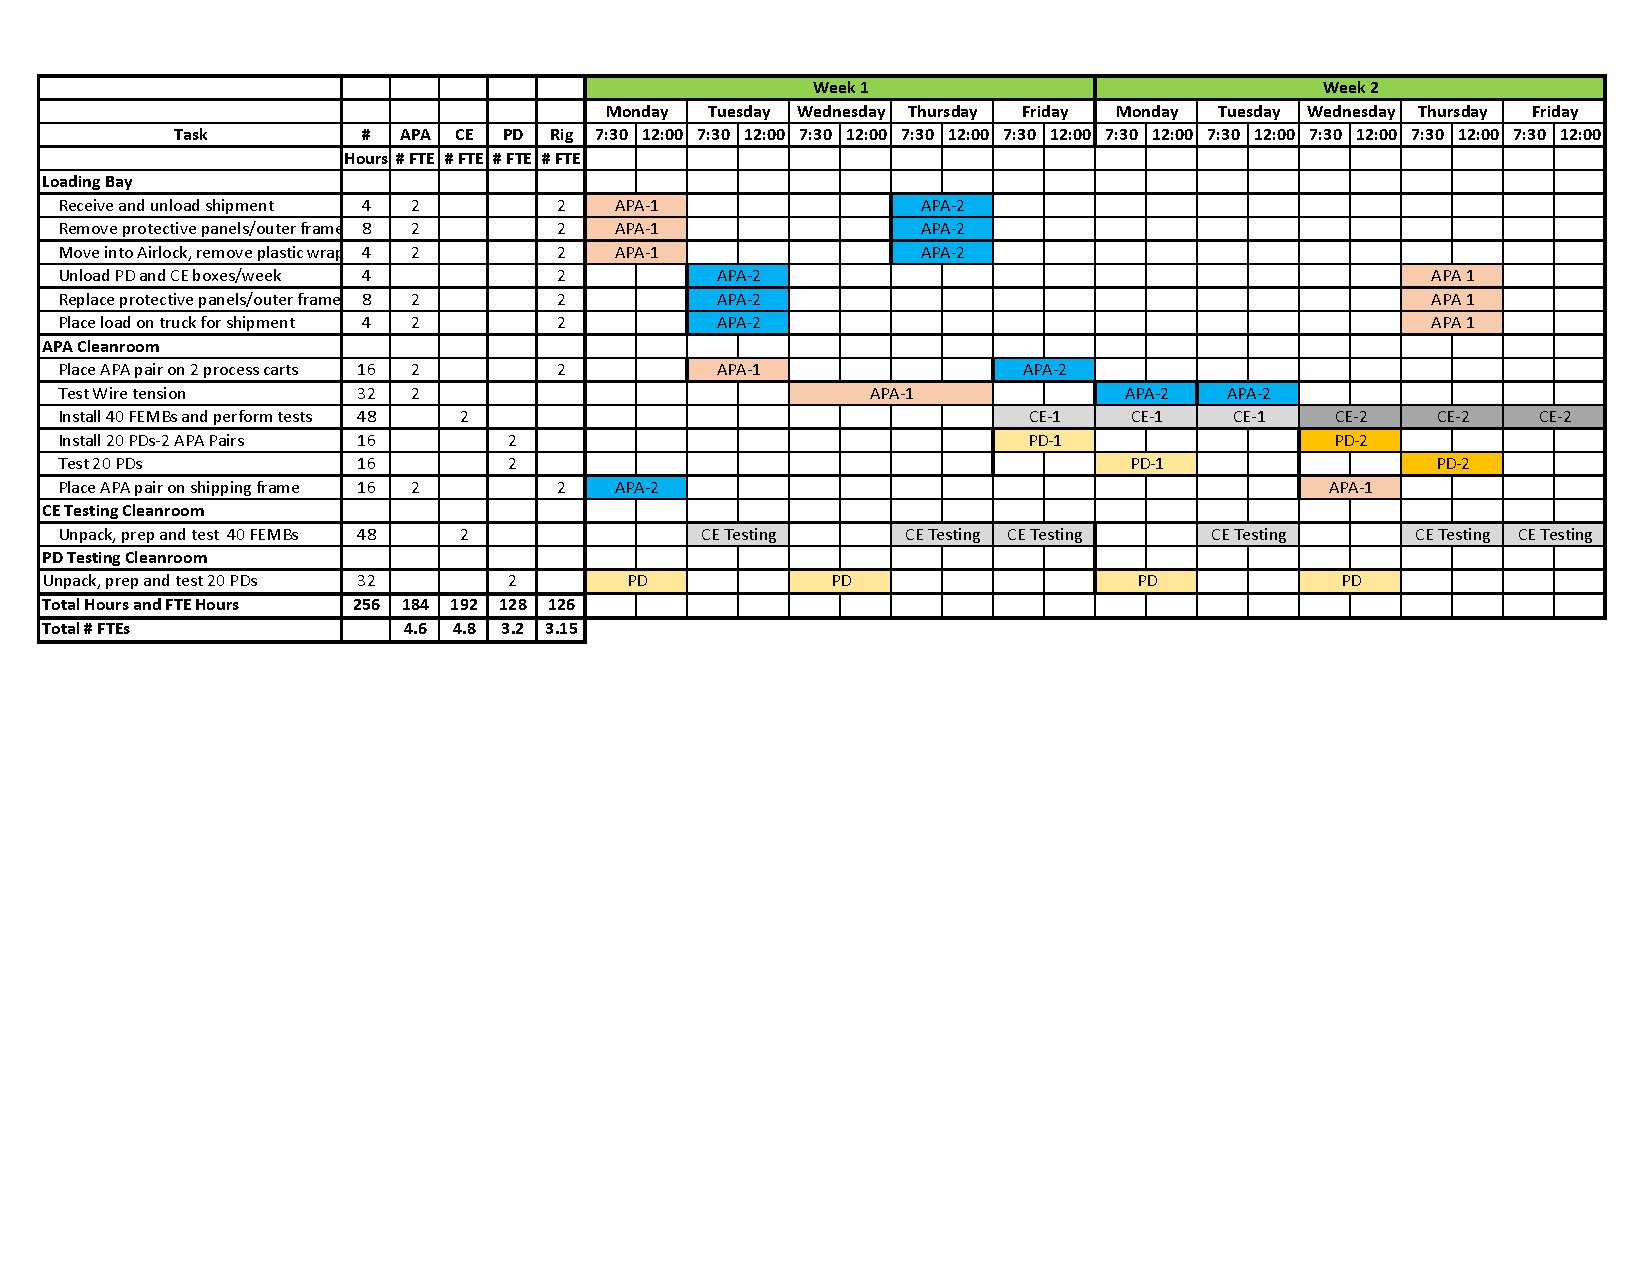
\includegraphics[width=0.98\textwidth]
{ITF-Schedule.pdf} 
\end{dunefigure}


\fixme{use templates from cost-risk-sched.tex file. Anne}
